\section{\texorpdfstring{SCADA a HMI}{SCADA a HMI}}

% =====================================================================================================================
	\begin{frame}
    \frametitle{HMI - lokální dohled}
		
		\textbf{H}uman \textbf{M}achine \textbf{I}nterface
		
		\begin{itemize}
			\item je ovládací rozhraní pro operátora určitého stroje:
			
			\begin{itemize}
				\item obrazovka,
				\item panel,
				\item aplikace,
			\end{itemize}
			\item často běží přímo na panelu u stroje.
		\end{itemize}

	\end{frame}
	

% =====================================================================================================================
	\begin{frame}
    \frametitle{SCADA - celkový dohled}
		
		\textbf{S}upervisory \textbf{C}ontrol and \textbf{D}ata \textbf{A}cquisition 
		
		\begin{itemize}
			\item celý systém nad \textbf{více zařízeními},
			\item sbírá data z jednotlivých PLC,
			\item ukládá historii, postmorty, řeší alarmy,
			\item poskytuje vizualizaci.
		\end{itemize}

	\end{frame}
	
% =====================================================================================================================
	\begin{frame}
    \frametitle{OPC server}
		
		\textbf{O}LE for \textbf{P}rocess \textbf{C}ontrol 
		
		\begin{center}
			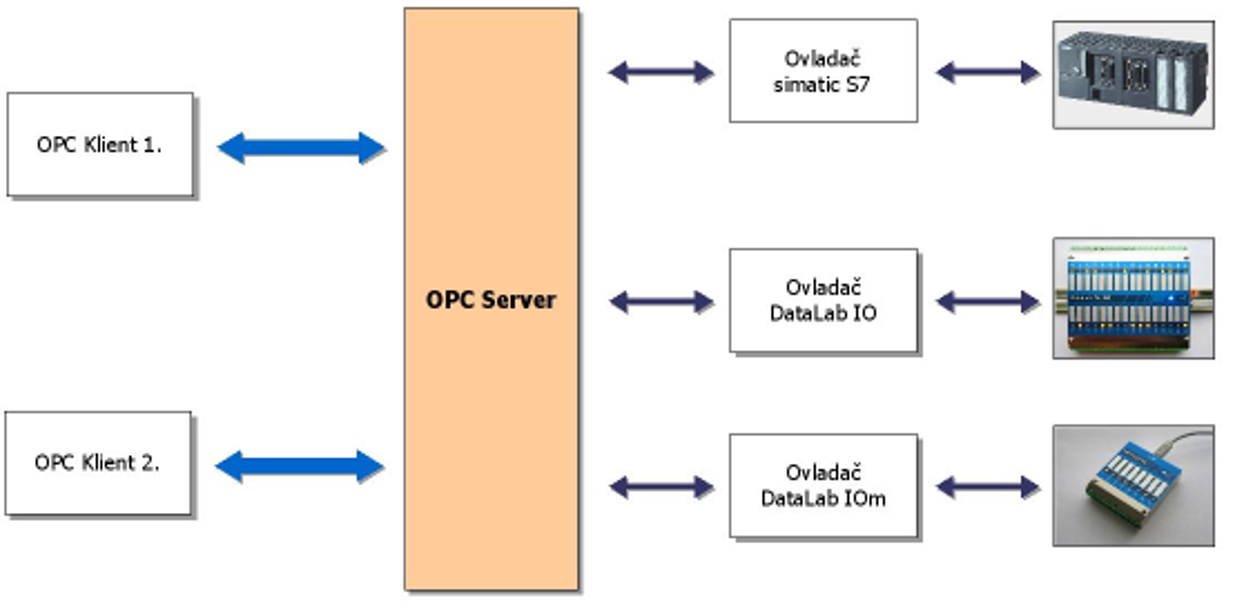
\includegraphics[width=1.00\textwidth]{fig/opc.png}
		\end{center}

	\end{frame}
	
% =====================================================================================================================
	\begin{frame}
    \frametitle{OPC server - poskytování dat}
		
		\textbf{Příklad:}
		
		\begin{itemize}
			\item PLC má vlastní způsob poskytování dat: MODBUS, MBUS, PROFIBUS, ...
			\item SCADA potřebuje data ve své formě, takto zjevně musí obsahovat určeného klienta podle typu komunikace.
		\end{itemize}
		
		\textbf{Řešení pomocí \textbf{OPC serveru}:}
		
		\begin{itemize}
			\item Externí OPC server se připojí do PLC pomocí určeného typu komunikace, nebo je OPC server přímo součástí PLC.
			\item OPC server získává data z PLC a ty vystavuje v podobě \textbf{uzlů} (= proměnné, uvidíme dále).
			\item Jakákoliv klientská SCADA se připojuje k OPC serveru, čte tyto uzly a zapisuje je například do HMI.
		\end{itemize}
		 

	\end{frame}
	
% =====================================================================================================================
	\begin{frame}
    \frametitle{OPC UA - přístup}
		
		\begin{itemize}
			\item Typicky běží na portu \textbf{4840},
			\item umožňuje procházení uzlů (\textbf{node}), tedy není nutné znát názvy uzlů dopředu, ale vyčtou se ze serveru,
			\item uzly mají stromovou strukturu (grupování dat),
			\item uzly mají různé třídy:
			
			\begin{itemize}
				\item Root - počátek stromu,
				\item Object - runtime data,
				\item Type - definice typů,
				\item Variable - proměnná, atd.
			\end{itemize}
		\end{itemize}
		 
	\end{frame}
	
% =====================================================================================================================
	\begin{frame}
    \frametitle{OPC UA - node, uzel}
		
		\begin{itemize}
			\item může jít o proměnnou, metodu, datový typ, ...
			\item základní atributy:
			
			\begin{itemize}
				\item \textbf{NodeId} je jednoznačný identifikátor pro komunikaci,
				\item \textbf{NodeClass} je typ (třída) uzlu,
				\item \textbf{BrowseName} je název ve stromě při procházení,
				\item \textbf{DisplayName} je název pro člověka $\Rightarrow$ lze lokalizovat,
				\item \textbf{Descripion} je popis,
			\end{itemize}
			\item další atributy jsou závislé na třídě, například \textbf{Variable} bude mít atribut \textbf{Value} s hodnotou.
		\end{itemize}
		
		Pro zajištění unikátnosti názvů se zavádí jmenný prostor - \textbf{namespace}:
		
		\begin{itemize}
			\item ns=0, rezervováno pro OPC UA standard, systémové uzly,
			\item ns=1, obvykle pro server, diagnostika,
			\item ns=2 a dále pro zařízení.
		\end{itemize}
		 
	\end{frame}